%!TEX root = ProgCPP_ZF.tex

%TODO weiter korrigieren

\part{Scope, Deklarationen, Type Casts}
\label{sec:Kapitel 5: Scope, Deklarationen, Type Casts}

% Unterabschnitt: Strukturen

\section{Strukturen in C++}
\label{sec:Strukturen in C++}
\begin{itemize}
	\item Grundsätzlich sind Strukturen in C++ identisch zu Strukturen in C
	\item In C++ haben Strukturen noch zusätzliche Möglichkeiten (folgt im Zusammenhang mit Klassen)
	\item Die Definition und Nutzung von Strukturen ist in C++ einfacher, typedef braucht es nicht
	\item[\-] 
	\noindent
\begin{minipage}{\linewidth}
\begin{lstlisting}
struct Point
{
	double x;
	double y;		
};
	
Point p1;
\end{lstlisting}
\end{minipage}
\end{itemize}

% Unterabschnitt: Gültigkeitsbereiche, Namensräume und Sichtbarkeit
\section{Gültigkeitsbereiche, Namensräume und Sichtbarkeit}
\label{sec:Gueltigkeitsbereiche, Namensraeume und Sichtbarkeit}

\subsection{Gültigkeitsbereiche von Namen (Scope)}
\label{sec:Gueltigkeitsbereiche von Namen (Scope)}
\begin{itemize}
	\item Prinzipiell identisch wie in C
	\item Der Compiler arbeitet immer Dateiweise
	\item Namen in einer anderen Datei sind dem Compiler nicht bekannt
	\item (Globale) Variablen, welche in einer anderen Datei definiert werden, können mit Hilfe des extern-Statements bekannt gemacht werden
	\item Durch das extern-Statement wird kein Speicherplatz reserviert
	\item[\-]
	\noindent
\begin{minipage}{\linewidth}
\begin{lstlisting}
extern int Foo_globalVariable;
\end{lstlisting}
\end{minipage}
	\item Funktionsprototypen und Definitionen, die von anderen Modulen genutzt werden können (Schnittstellen), werden in einer Headerdatei definiert
	\item Durch \#include der Headerdatei wird der Header geladen und die Namen bekannt gemacht
\end{itemize}

\subsection{Gültigkeitsbereiche in C++}
\label{sec:Gueltigkeitsbereiche in C++}
\begin{itemize}
	\item Lokaler Gültigkeitsbereich (local scope)
	\item[\-] Alle in einem Block deklarierten Bezeichner gelten von ihrer Deklaration an bis zum Ende des aktuellen Blocks
	\item Gültigkeitsbereich Funktionsprototyp, Funktion
	\item[\-] Alle in einem Funktionskopf deklarierten Bezeichner (Parameter) gelten in der gesamten Funktion
	\item Gültigkeitsbereich Namensraum (namespace)
	\item[\-] Alle im Namensraum deklarierten Bezeichner gelten von ihrer Deklaration an bis zum Ende des Namensraums
	\item Gültigkeitsbereich Klasse
	\item[\-] Alle in einer Klasse deklarierten Bezeichner gelten von ihrer Deklaration an in der gesamten Klasse
\end{itemize}

\subsection{Gültigkeit (Scope) von Variablen}
\label{sec:Gueltigkeit (Scope) von Variablen}
\begin{itemize}
	\item Eine Variable ist an einer bestimmten Stelle gültig, wenn ihr Name an dieser Stelle dem Compiler durch eine Vereinbarung bekannt ist
	\item Gültige Variablen können für den Programmierer unsichtbar sein, wenn sie durch eine andere Variable desselben Namens verdeckt werden
\end{itemize}

\subsection{Lebensdauer von Variablen}
\label{sec:Lebensdauer von Variablen}
\begin{itemize}
	\item Die Lebensdauer ist die Zeitspanne, in der das Laufzeitsystem des Compilers der Variablen einen Platz im Speicher zur Verfügung stellt
	\item Mit anderen Worten, während ihrer Lebensdauer besitzt eine Variable einen Speicherplatz
	\item Globale Variablen leben solange wie das Programm
	\item Lokale Variablen werden beim Aufruf des Blocks angelegt und beim Verlassen des Blocks wieder (automatisch!) ungültig
\end{itemize}

\subsection{Sichtbarkeit von Variablen}
\label{sec:Sichtbarkeit von Variablen}
\begin{itemize}
	\item Variablen von inneren Blöcken sind nach aussen nicht sichtbar
	\item Globale Variablen und Variablen in äusseren Blöcken sind in inneren Blöcken sichtbar
	\item Werden lokale Variablen mit demselben Namen wie eine globale Variable oder wie eine Variable in einem umfassenden (äusseren) Block definiert, so ist innerhalb des Blockes nur die lokale Variable sichtbar. Die globale Variable bzw. die Variable in dem umfassenden Block wird durch die Namensgleichheit verdeckt.
\end{itemize}

\subsection{Schlussfolgerung (naheliegend aber falsch)}
\label{sec:Schlussfolgerung (naheliegend aber falsch)}
\begin{itemize}
	\item Alle Variablen global definieren, dann muss ich mir keine Sorgen um die Sichtbarkeit machen
\end{itemize}
$\rightarrow$ Stimmt schon, aber:
\begin{itemize}
	\item Weil die Variablen in demselben Namensraum sind, müsste ich die Variablennamen im gesamten Projekt abstimmen
	\begin{itemize}
		\item[\-] $\rightarrow$ ist nicht praktikabel
	\end{itemize}
	\item Globale Variablen haben gewichtige Nachteile: Wer hat den Variablenwert wo wie geändert?
	\begin{itemize}
		\item[\-] $\rightarrow$ schwer nachzuvollziehen
	\end{itemize}
\end{itemize}

\subsection{Lebensdauer (grau) und Sichtbarkeit (weiss)}
\label{sec:Lebensdauer (grau) und Sichtbarkeit (weiss)}
\noindent
\begin{figure}[hh]
	\centering
	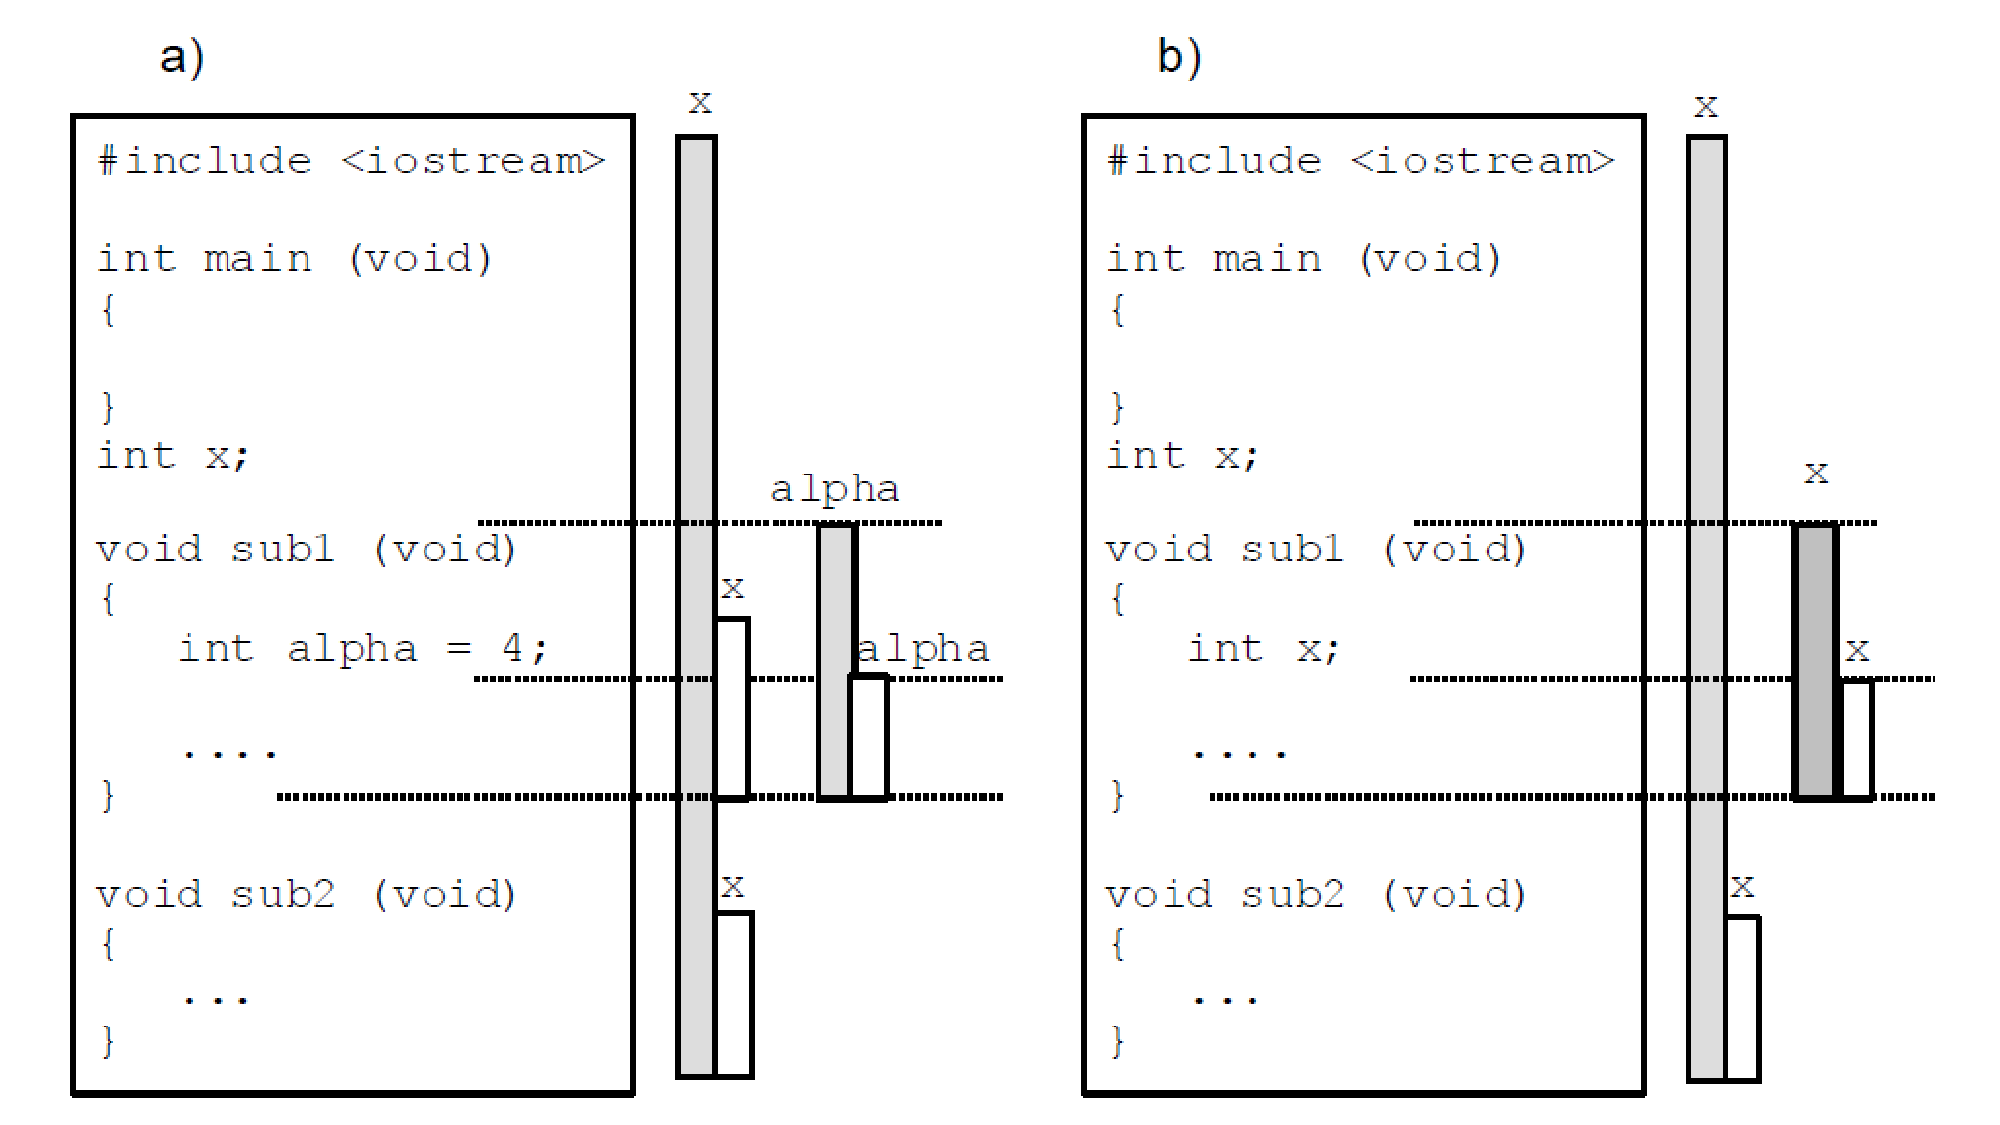
\includegraphics[width=0.7\linewidth]{images/scope1.pdf}
\end{figure}

\subsection{Codierstil}
\label{sec:Codierstil}
\begin{itemize}
	\item Variablen so lokal wie möglich definieren, d.h. im innersten möglichen Block (Tipp: nur am Anfang eines Blocks)
	\item Globale Variablen wenn immer möglich vermeiden. Sie müssen speziell gekennzeichnet werden. Sie sollen (in C) mit einem Prefix (Modulkürzel) gefolgt von einem underscore character (\_) beginnen. Dadurch werden die Namen eindeutig.
	\item[\-] Beispiel:\\Die globale Variable counter im Modul Foo muss wie folgt definiert werden:
	\noindent
\begin{minipage}{\linewidth}
\begin{lstlisting}
int Foo_counter;
\end{lstlisting}
\end{minipage}
	\item Globale Variablen am Anfang der Datei definieren, d.h. auf jeden Fall vor der ersten Funktion
\end{itemize}
\begin{hinweis}
Besser (in C++): Namespace definieren
\end{hinweis}

% Unterkapitel: Namensräume (Namespaces)

\section{Namensräume (Namespaces)}
\label{sec:Namensraeume (Namespaces)}
\textbf{Namen, die zu verschiedenen Namensräumen gehören, dürfen auch innerhalb desselben Gültigkeitsbereichs gleich sein.}
In C gibt es die folgenden Namensräume (gilt auch für C++):
\begin{itemize}
	\item Marken
	\item Namen von Strukturen, Unions und enums
	\item Jede Struktur und Union für ihre Feldnamen
	\item Bezeichner von Variablen, Funktionen, typedef-Namen, enum-Konstanten
\end{itemize}
In C++ können zusätzlich explizit definierte Namensräume verwendet werden.\\
\begin{hinweis}
Dadurch können (und sollen unbedingt!) die in C üblichen Modulkürzel vermieden werden.
\end{hinweis}

\subsection{Explizite Namensräume in C++}
\label{sec:Explizite Namensraeume in C++}
\begin{itemize}
	\item Nebst den vordefinierten (impliziten) Namensräumen des vorherigen Abschnitts können in C++ explizit eigene Namensräume (namespaces) definiert werden.
	\item Bezeichner müssen nur innerhalb ihres Namensraums eindeutig sein
	\item Für jedes Modul in C (mit Modulkürzel) soll in C++ ein Namensraum definiert werden
	\item Sie haben bisher in allen C++-Übungen bereits den Namensraum std verwendet
\end{itemize}

\subsection{C++-Mechanismen für Namespaces}
\label{sec:C++-Mechanismen fuer Namespaces}
\begin{itemize}
	\item Deklaration von Namespaces
	\item Namespace-Alias
	\item[\-] Einem bestehenden Namespace einen anderen Namen zuweisen (eher selten)
\noindent
\begin{minipage}{\linewidth}
\begin{lstlisting}
namespace fbssLib = financial_branch_and_system_service_library;
\end{lstlisting}
\end{minipage}
	\item using-Deklaration
	\item using-Direktive
\end{itemize}

\subsection{Deklaration von Namespaces}
\label{sec:Deklaration von Namespaces}
\begin{itemize}
	\item Alle in einem Namespace deklarierten Bezeichner werden diesem Namespace zugeordnet
	\item Auf die Bezeichner des Namespaces kann mit dem Scope-Operator :: zugegriffen werden
	\item Syntax:
	\item[\-] Hinter dem Schlüsselwort namespace folgt der Name des Namespaces gefolgt von einem Block
	\item Innerhalb einer Datei kann mehr als ein Namespace deklariert werden (eher unüblich) und ein Namespace kann in mehreren Dateien deklariert sein (häufig, d.h. die Elemente eines Namespaces werden in mehreren Dateien implementiert)
\end{itemize}

\subsubsection{Beispiel}
\label{sec:Deklaration von Namespaces: Beispiel}
\noindent
\begin{minipage}{\linewidth}
\begin{lstlisting}
namespace myLib1
{
	int i;
	void foo();
}

namespace myLib2
{
	int i;
	void foo();
	int go();
}

...
{
	myLib1::foo();	// vollstaendiger Name von foo()
	myLib2::i = 17;	// vollstaendiger Name von i
}
\end{lstlisting}
\end{minipage}

\subsection{using-Deklaration}
\label{sec:using-Deklaration}
\begin{itemize}
	\item Eine using-Deklaration ''importiert'' Namen aus einem Namensraum und macht ihn ohne explizite Namensraumangabe verwendbar
	\item Sie kann lokal in einem Block oder global ausserhalb eines Blocks verwendet werden
	\item Deklariert nur einzelne Namen
\end{itemize}
\noindent
\begin{minipage}{\linewidth}
\begin{lstlisting}
int main()
{
	using myLib1::foo;	// lokales Synonym
	foo();			// ruft myLiby::foo() auf
}
\end{lstlisting}
\end{minipage}

\subsection{using-Direktive}
\label{sec:using-Direktive}
\begin{itemize}
	\item Eine using-Direktive macht alle Namen aus einem Namensraum ohne explizite Namensraumangabe verwendbar
\end{itemize}
\noindent
\begin{minipage}{\linewidth}
\begin{lstlisting}
usting namespace myLib1;	// ''importiert'' alle Namen aus myLib1

int main()
{
	foo();			// ruft myLib1::foo() auf
}
\end{lstlisting}
\end{minipage}

\subsection{using namespace kann zu Konflikten führen}
\label{sec:using namespace kann zu Konflikten fuehren}
\begin{itemize}
	\item Wenn bei mehreren using namespace-Deklarationen und/oder -Direktiven die Namen (ohne Namespace-Angabe) nicht eindeutig sind, müssen die Namen voll qualifiziert verwendet werden (mit Namespace-Angabe)
\end{itemize}
\noindent
\begin{minipage}{\linewidth}
\begin{lstlisting}
namespace myLib1
{
	int i;
	void foo();
}

namespace myLib2
{
	int i;
	void foo();
	int go();
}

...
{
	myLib1::foo();	*@\color{red}//ist nicht eindeutig, Compiler reklamiert@*
	myLib2::i = 17;	// vollstaendiger Name von i
}
\end{lstlisting}
\end{minipage}

\subsection{Namenlose Namespaces}
\label{sec:Namenlose Namespaces}
\begin{itemize}
	\item Ein namenloser Namespace wird wie ein spezieller Namensraum mit einem systemweit eindeutigen Namen behandelt
\end{itemize}
\begin{hinweis}
Es ist guter Programmierstil, den Gültigkeitsbereich aller nur intern verwendeten Funktionen und Daten mit Hilfe von namenlosen Namespaces auf den Bereich eingrenzen, in dem die Objekte verwendet werden. (In C hat man dafür die Funktionen mit static gekennzeichnet
\end{hinweis}
\noindent
\begin{minipage}{\linewidth}
\begin{lstlisting}
namespace
{


}
\end{lstlisting}
\end{minipage}

\subsection{Zugriff auf globale Variable mit Scope-Operator}
\label{sec:Zugriff auf globale Variable mit Scope-Operator}
\noindent
\begin{minipage}{\linewidth}
\begin{lstlisting}
int zahl = 11;	// globale Variable

int main()
{
	int zahl = 22;		// lokale Variable
	zahl = zahl + 4;	// lokale Variable
	::zahl = 23;		// Zugriff auf globale Variable
}
\end{lstlisting}
\end{minipage}

% Unterabschnitt: Speicherklassen

\section{Speicherklassen}
\label{sec:Speicherklassen}

\subsection{Speicherklassen in C++}
\label{sec:Speicherklassen in C++}
\begin{itemize}
	\item auto
	\item[\-] Ist default, wenn nichts geschrieben wird. Eine mit auto deklarierte Variable wird nach Beendigung des Scopes automatisch entfernt.\\
	Achtung: hat ab C++11 eine andere Bedeutung!!
	\item register
	\item[\-] Ist dasselbe wie auto mit zusätzlichem Hinweis an Compiler: wenn es geht in ein Register legen (sehr zurückhaltend einsetzen, besser gar nicht)
	\item static
	\item extern
	\item mutable
	\item[\-] (später im Zusammenhang von Klassen)
\end{itemize}

\subsubsection{Speicherklasse static: Variablen}
\label{sec:Speicherklasse static: Variablen}
\begin{itemize}
	\item static-Variablen sind im Datenbereich, nicht auf dem Stack
	\item Sie werden automatisch auf 0 initialisiert, wenn nichts anderes steht
	\item Gültigkeitsbereich ist der Block, in dem die Variable definiert ist
	\item static-Variablen, welche ausserhalb einer Funktion definiert sind (globale Variablen). sind nur in der Datei gültig, in der sie definiert werden
	\item static-Variablen sind nur einmal vorhanden (auch in multi-threading-Umgebungen), d.h. ihr Wert wird erhalten, auch wenn die Funktion beendet ist. Beim nächsten Aufruf der Funktion geht es mit dem alten Wert weiter.\color{red}
	\item Nur einsetzen, wenn man das will!\color{black}
\end{itemize}

\subsubsection{Speicherklasse static: Funktionen}
\label{sec:Speicherklasse static: Funktionen}
\begin{itemize}
	\item static-Funktionen sind nur in der Datei, in welcher sie definiert sind, sichtbar
	\item Alle Funktionen, welche nicht aussen (für andere Units) sichtbar sein sollen, sollten deshalb \textbf{in C} als static definiert werden\color{red}
	\item In C++ können dafür namenlose Namespaces verwendet werden (bevorzugt)\color{black}
\end{itemize}

\subsubsection{Speicherklasse extern: Externe Variablen}
\label{sec:Speicherklasse extern: Externe Variablen}
\begin{itemize}
	\item Eine externe Variable kann nur in einer einzigen Datei definiert werden (ohne Speicherklasse extern)
	\item In den anderen Dateien wird sie mit extern deklariert (bekannt gemacht)
	\item Eine manuell Initialisierung ist nur bei der Definition möglich
	\item Globale Variablen, welche nicht manuell initialisiert werden, werden automatisch mit 0 initialisiert
	\item extern-Deklarationen werden üblicherweise in einer Headerdatei deklariert und am Beginn der Datei mit \#include eingefügt
\end{itemize}

\subsection{Typqualifikationen (Kap. 9.2.2)}
\label{sec:Typqualifikationen (Kap. 9.2.2)}
\begin{itemize}
	\item const
	\item[\-] const-Objekte können nicht verändert werden (read-only)
	\item volatile
	\item[\-]Der Compiler wird angewiesen, keine Optimierungen (soweit sie die Variable betreffen) vorzunehmen
	\item volatile wird oft bei Embedded Systems angewandt, wenn z.B. ''hinter'' einer Variable ein Register liegt.
	\item const und volatile können auch kombiniert werden, z.B. bei read-only-Hardwareregistern
\end{itemize}

\subsection{Funktionsattribute}
\label{sec:Funktionsattribute}
\begin{itemize}
	\item inline
	\item[\-] bereits bekannt
	\item virtual
	\item[\-] später im Zusammenhang mit Klassen
	\item explicit
	\item[\-] später im Zusammenhang mit Klassen
\end{itemize}

% Unterkapitel: Typdefinitionen

\section{Typdefinitionen}
\label{sec:Typdefinitionen}

\subsection{typedef zur Vereinbarung eigener Datentypen\hfill}
\label{sec:typedef zur Vereinbarung eigener Datentypen}
\begin{itemize}
	\item analog C
	\item In C++ kann aber z.B. bei structs das typedef weggelassen werden
	\item In C:
	\item[\-]
\noindent
\begin{minipage}{\linewidth}
\begin{lstlisting}
typedef struct {int x;
		iny;} Point;
\end{lstlisting}
\end{minipage}
	\item In C++:
	\item[\-]
\noindent
\begin{minipage}{\linewidth}
\begin{lstlisting}
struct Point {
	int x;
	int y;
};
\end{lstlisting}
\end{minipage}
	\item Stil: eigene Typen werden mit einem Grossbuchstaben begonnen
\end{itemize}

\subsubsection{Beispiel}
\label{sec:Beispiel}
\noindent
\begin{minipage}{\linewidth}
\begin{lstlisting}
struct Point {
	int x;
	int y;
};

struct Line {
	Point p1;
	Point p2;
};

int main(void)
{
	line myLine = {12, -34,		// p1
			783, 12};	// p2
		
	std::cout << ''Startpunkt: ('' << myLine.p1.x << '', ''
					<< myLine.p1.y << '')\n'';
	std::cout << ''Endpunkt: ('' << myLine.p2.x << '', ''
					<< myLine.p2.y << ''\n'';
	return 0;
}
\end{lstlisting}
\end{minipage}

\subsection{Gewährleistung von Portabilität}
\label{sec:Gewaehrleistung von Portabilitaet}
\begin{itemize}
	\item Oft muss z.B. ein Register ein 16 Bit breiter Wert geschrieben werden. Welcher Typ ist nun 16 Bit breit?
	\item Das ist implementationsabhängig (vielleicht unsigned short, unsigned int, ...)
	\item Um die Portabilität (Umschrieben auf ein anderes System) zu vereinfachen, wird ein 16 Bit breiter Datentyp (Word) definiert und dann ausschliesslich verwendet (in stddef.h sind diese Typen üblicherweise bereits definiert). Auf einem anderen System ist dann nur noch dieser typedef zu ändern.
	\item[\-] 
\noindent
\begin{minipage}{\linewidth}
\begin{lstlisting}
typedef unsigned short uint16_t;
\end{lstlisting}
\end{minipage}
\end{itemize}

\subsection{Wie setzt der Compiler ein typedef um?}
\label{sec:Wie setzt der Compiler ein typedef um?}
\begin{itemize}
	\item Ein typedef ist mehr oder weniger eine reine Textersetzung. Erklärung anhand des folgenden Beispiels:
	\item[\-]
\noindent
\begin{minipage}{\linewidth}
\begin{lstlisting}
typedef struct {int x;
		int y;} Point;
\end{lstlisting}
\end{minipage}
	\item Überall im Code, wo nun das Wort Point gefunden wird, ersetzt der Compiler dieses in einem ersten Durchgang mit dem Text 
	\item[\-]
\noindent
\begin{minipage}{\linewidth}
\begin{lstlisting}
typedef struct {int x;
		int y;}
\end{lstlisting}
\end{minipage}	
\end{itemize}

\section{Initialisierung}
\label{sec:Initialisierung}
\begin{itemize}
	\item analog C
\end{itemize}

\section{Type-Cast (Typumwandlungen)}
\label{sec:Type-Case (Typumwandlungen)}

\subsection{Typumwandlungen im Allgemeinen}
\label{sec:Typumwandlungen im Allgemeinen}
\begin{itemize}
	\item Unsafe conversion
	\item[\-] Wenn bei der Typumwandlung signifikante Stellen verloren gehen können (typischerweise bei einer Umwandlung von einem ''grösseren'' in einen ''kleineren'' Typ, z.B. von double nach int)
	\item[\-] Bei int ist siwihl die Genauigkeit als auch die maximal darstellbare Zahl
	\item Safe conversion
	\item[\-] Wenn bei der Typumwandlung keine signifikanten Stellen verloren gehen können (typischerweise bei einer Umwandlung von einem ''kleineren'' in einen ''grösseren'' Typ, z.B. von in nach double
\end{itemize}

\subsection{Implizite Typumwandlung}
\label{sec:Implizite Typumwandlung}
\begin{itemize}
	\item Die implizite (automatische) Typumwandlung wird auch als Standard-Typumwandlung bezeichnet
	\item Sie erfolgt analog zur Programmiersprache C (siehe dort)
\end{itemize}

\subsection{Explizite Typumwandlung}
\label{sec:Explizite Typumwandlung}
\begin{itemize}
	\item Nebst den impliziten (automatischen) Typumwandlungen kann in C++ mit Hilfe von 6 verschiedenen cast-Operatoren eine explizite Typumwandlung bewirkt werden.
	\item Bei der expliziten Typumwandlung gibt der Programmierer explizit an, was er will.
	\item[\-]
	\begin{achtung}
	Bei der expliziten Typumwandlung übernimmt der Programmierer die Verantwortung, dass die Umwandlung keine Probleme ergibt.\\
	(z.B. Umwandlung von grosser Zahl in kleineren Typ)
	\end{achtung}
\end{itemize}

\subsubsection{Explizite Typumwandlung \#1, 2: C-Stil und Funktionsstil}
\label{sec:Explizite Typumwandlung 1}
\begin{itemize}
	\item Stroustrup: ''The C and C+ cast is a sledgehammer...''
	\item Syntax für C-Stil (einzige Variante in C):
	\item[\-](Zieltyp)expression
	\item[\-]
\noindent
\begin{minipage}{\linewidth}
\begin{lstlisting}
int a = (int)4.6;	// a == 4
\end{lstlisting}
\end{minipage}
	\item Syntax für Funktionsstil:
	\item[\-] Zieltyp(expression)
	\item[\-]
\noindent
\begin{minipage}{\linewidth}
\begin{lstlisting}
int a = int(4.6);	// a == 4
\end{lstlisting}
\end{minipage}
\end{itemize}

\subsubsection{Typumwandlung mit C-Stil und Funktionsstil}
\label{sec:Typumwandlung mit C-Stil und Funktionsstil}
\textbf{Typumwandlung ist...}
\begin{itemize}
	\item einfache Reinterpretation der bitweisen Darstellung des Ausdrucks
	\item einfache arithmetische Grössenanpassung
	\item ein const- oder volatile-Attribut zu einem Ausdruck hinzufügen oder entfernen
	\item andere (eventuell implementierungsabhängige) Umwandlung
\end{itemize}
\begin{achtung}
Aus dem Sourcecode geht nicht hervor, welche der aufgeführten Typumwandlungen der Programmierer wollte.\\ 
Diese beiden Casts sollten in C++ nicht verwendet werden!
\end{achtung}

\subsubsection{Explizite Typumwandlung \#3: const\_cast}
\label{sec:Explizite Typumwandlung 3}
\textbf{Anwendung:}\\
Ausschliesslich die (vorübergehende) Entfernung des const-Qualifikators, d.h. die Umwandlung eines Ausdrucks vom Typ T mit den optionalen Qualifikatoren const und volatile in einen Ausdruck desselben Typs ohne den Qualifikator const\\
\textbf{Syntax:}
\noindent
\begin{minipage}{\linewidth}
\begin{lstlisting}
const_cast<Zieltyp>expression

const char* findSubString(const char* str, const char* subStr)
{
	return strstr(const_cast<char*<str,
			const_cast<char*>subStr);
}
\end{lstlisting}
\end{minipage}
Die Funktion strstr() akzeptiert nur Parameter com Typ char* (ohne const)

\subsubsection{Explizite Typumwandlung \#4: static\_cast}
\label{sec:Explizite Typumwandlung 4}
\textbf{Anwendung:}\\
Umwandlung von Objekten einer Klasse auf Objekte einer Basisklasse oder die Umwandlung mittels einer Umwandlungsfunktion.\\
Wenn schon Type cast, dann ist static\_cast die häufigste.

\subsubsection{Explizite Typumwandlung \#5: dynamic\_cast}
\label{esc:Explizite Typumwandlung 5}
\textbf{Anwendung:}\\
Umwandlung von polymorphen Objekten im Zusammenhang mit dem Typsystem von C++ eingesetzt (Stichwort RTTI = Runtime Type Information System)\\
Näheres folgt später im Zusammenhang mit Klassen und Polymorphismus.

\subsubsection{Explizite Typumwandlung \#6: reinterpret\_cast}
\label{sec:Explizite Typumwandlung 6}
\textbf{Anwendung:}\\
reinterpret\_cast ist eine neue Interpretation der zugrunde liegenden Bitkette.\\
\textbf{Syntax:}
\noindent
\begin{minipage}{\linewidth}
\begin{lstlisting}
reinterpret_cast<Zieltyp>expression

char* p = new char[20];
...
int* pi = reinterpret_cast<int*>p;
\end{lstlisting}
\end{minipage}


